
\section{Evaluation}
\label{sect:exper}

We have implemented and evaluated a prototype of our VC scheme on a Linux cluster of machines with
8-core AMD FX-8120 at 3.1 GHz with 16 GB RAM. 
Our implementation is based on Alibaba's Xen cloud platform~\cite{Aliyun,WeiZhangIEEE}.
Each machine  is equipped with a 
a distributed file system (QFS) and overall the cluster manages six 3TB disks
with default replication degree set to 3. The PDS replication is set to 5.
Objectives of our evaluation are:
1) Study the duplicate detection and removal effectiveness of the VC approach and compare with an alternative VO
design.
2) Examine the impacts of VC for fault isolation and tolerance. 
3) Evaluate the backup throughput performance VC  for a large number of VMs.
4) Assess the resource usage  of VC in terms of memory, storage, and network bandwidth.
% the backup throughput performance VC  for a large number of VMs.
%Compare with the data domain approach~\cite{bottleneck08}.

%\section{Experiments}
%Our main test-bed is an cluster of 6 machines,
%Our data set consists of 350 virtual machine image snapshots taken from Alibaba.com's
%public VM cloud in China. 
%We select 35 VMs from the most popular 7 OSes: 
%Debian, Ubuntu, Redhat, CentOS, Win2003 32bit, win2003 64 bit and win2008 64 bit. 
%For each OS, 5 VMs are chosen, and every VM come with 10 full snapshots.
%\subsection{Experimental setup}

We will also compare our VC approach with  with
a VO approach  using stateless routing with binning (SRB).
SRB executes a distributed deduplication by routing a data chunk to a machine~\cite{ParallelDataDomain}
using  the chunk hashing function discussed in \cite{??}. Within such a machine,
the data chunk is compared with a local index. This minHash paritioning
algorithm helps provide a greater degree of parallelism, but ignores the
significant amount of parallelism within a single VM.

\comments{
%We are running our deduplication/backup  service on 100 nodes.
%Memory usage is about 150MB space per node during backup and
%the CPU usage is very small during the experiments. 
We have performed a trace-driven study using  a 1323 VM dataset  collected from 
%100 Alibaba Aliyun's cloud nodes~\cite{WeiZhangIEEE}.
a cloud cluster at Alibaba's Aliyun.
 ~\cite{WeiZhangIEEE}.
% and each of machine nodes has 16 cores and 12 disk drives,  hosting  up to 25 VMs. 
For each VM, the system keeps 10 automatically-backed snapshots in the storage while
a user may instruct extra snapshots to be saved.
Each VMs uses   one of the most popular 7 OSes: 
Debian, Ubuntu, Redhat, CentOS, Win2003 32bit, win2003 64 bit and win2008 64 bit. 
The backup of VM snapshots is completed within a few  hours every night.
Based on our study of production  data,  each VM has about  40GB of storage  data on average
including OS and user data disk.
For our system each VM image is  divided into 2 MB fix-sized segments and each segment is divided into 
variable-sized content blocks  with an average size of 4KB.
%variable sizes~\cite{similar94,rabin81} with an average size of 4KB. 
The signature for variable-sized blocks is computed using their SHA-1 hash. 

The seek cost of each random IO request in our test machines is about  10 milliseconds.
The average I/O usage of local storage is controlled to about 50MB/second for backup 
in the presence of other I/O jobs. Noted that a typical 1U server can host
6 to 8  hard drives and deliver over 300MB/second. Our setting uses 16.7\% or less 
of local storage bandwidth. 
The final snapshots are stored in a distributed file system built on the same 
cluster. total local disk usage on each machine is about 8GB for the duplicate detection purpose,
mainly for global index. 
Level 1 segment dirty bits identify 78\% of duplicate blocks. For the remaining dirty segments,
block-wise full deduplication removes about additional 74.5\% of duplicates.
The final content copied to the backup storage is reduced by 94.4\%
\emph{Is this correct? Elsewhere we have used 92\% based on results from
our srb-vc comparison graph} in total.
}
%\begin{figure}
%\centering
%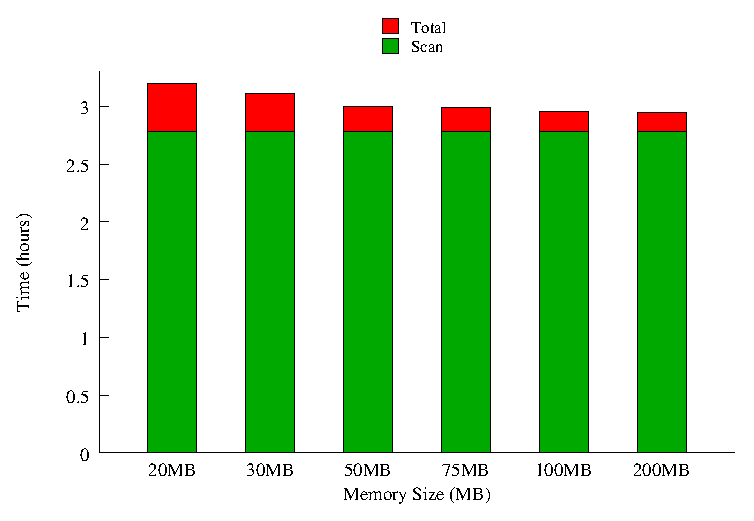
\includegraphics[width=0.4\textwidth]{mem_time}
%\caption{ Parallel time when memory limit varies.}
%\label{fig:memory}
%%\end{figure}
%
%Figure~\ref{fig:memory} shows the total parallel time in hours to backup 2500 VMs on
% a 100-node cluster a  when 


\subsection{Settings}
We have performed a trace-driven study using  a 1323 VM dataset  collected from 
100 Alibaba Aliyun's cloud nodes~\cite{WeiZhangIEEE}.
The production environment tested has  about 1000 machines with 25 VMs on each machine.
%We are running our deduplication/backup  service on 100 nodes.
%Memory usage is about 150MB space per node during backup and
%the CPU usage is very small during the experiments. 
% and each of machine nodes has 16 cores and 12 disk drives,  hosting  up to 25 VMs. 
For each VM, the system keeps 10 automatically-backed snapshots in the storage while
a user may instruct extra snapshots to be saved.
%Each VM uses   one of the most popular 7 OSes: 
%Debian, Ubuntu, Redhat, CentOS, Win2003 32bit, win2003 64 bit and win2008 64 bit. 
The backup of VM snapshots is completed within a few  hours every night.
Based on our study of production  data,  each VM has about  40GB of storage  data  on average
including OS and user data disk.
All data are divided into 2 MB fix-sized segments and each segment is divided into 
variable-sized content chunks ~\cite{similar94,rabin81} with an average size of 4KB.
The signature for variable-sized blocks is computed using their SHA-1 hash. 
Popularity of data blocks are collected through global counting 
and the top 1-2\% will fall into the PDS, as discussed in Section~\ref{sect:crossVM}.
%variable sizes~\cite{similar94,rabin81} with an average size of 4KB. 
%The signature for variable-sized blocks is computed using their SHA-1 hash. 

%The seek cost of each random IO request in our test machines is about  10 milliseconds.
%The average I/O usage of local storage is controlled about 50MB/second for backup 
%in the presence of other I/O jobs. Noted that a typical 1U server can host
%6 to 8  hard drives and deliver over 300MB/second. Our setting uses 16.7\% or less 
%of local storage bandwidth. 
%The final snapshots are stored in a distributed file system built on the same 
%cluster. 

%Level 1 segment dirty bits identify 78\% of duplicate blocks. For the remaining dirty segments,
%block-wise full deduplication removes about additional 74.5\% of duplicates.
%The final content copied to the backup storage is reduced by 94.4\% in total.
%Based on the data studied,  each VM has about  40GB of storage  data usage on average,
%OS disk and data disk each takes about 50\% of storage space.
%The backup of VM snapshots is completed within two hours every day,
%and that translates to a backup throughput of 139GB per second, or 500TB per hour.
%For each VM, the system keeps 10 automatically-backed snapshots in the storage while
%a user may instruct extra snapshots to be saved.

% the system must finish saving daily snapshots of all VMs in 2 hours. In our typical 1000 nodes cluster, each node hosts 25 VMs, each VM has 40GB of data on average, that translates to backup throughput of 139GB/second, or 500TB/hour.

%In our snapshot deduplication architecture, PDS is the key to achieve greater deduplication than
%incremental backup solutions. Our basic assumption of PDS us that VM disks, especially OS disks,
%have huge amount of data in common, and such common data can be represented by a relatively smaller data set
%because of their high appearence frequency. As a result, the major portion of snapshot deduplication effect shall 
%emerge from eliminating the duplication of such a small data set. In this section, we evaluate
%the effectiveness of PDS using real user VM disks from our production VM cluster.

Since it's impossible to perform large scale analysis without affecting production VM performance,
we sampled two data sets from real user VMs to measure the effectiveness of our deduplication scheme.
Dataset1 is used study the detail impact of 3-level deduplication process,
it compose of 35 VMs from 7 popular OSes: 
Debian, Ubuntu, Redhat, CentOS, Win2003 32bit, win2003 64 bit and win2008 64 bit. For each OS, 
5 VMs are chosen, and every VM come with 10 full snapshots of it OS and data disk. 
The overall data size for these 700 full snapshots is 17.6 TB.

Dataset2 contains the first snapshots of 1323 VMs' data disks from a small cluster with 100 nodes. 
Since inner-VM deduplication is not involved in the first snapshot, this data set helps us to 
study the PDS deduplication against user-related data. The overall size of dataset2 is 23.5 TB.

\subsection{Impact on Fault Tolerance}

Figure~\ref{fig:vm-availability} shows the reliability of VM backups as storage
nodes fail for different amounts of sharing of filesystem blocks in the index.
We show 6.3 for the VO sharing because that is what we measured in our dataset,
and while we expect it to continue to grow (thereby decreasing fault
tolerance), it should do so slowly, so we treated VO FSB sharing as a
contstant factor of 6.3, as it doesn't change our results. for VC we use 1250, because that is what we
estimate at 2500 VMs based on the linear growth up to 105 VMs. We also show
2500 VMs sharing each PDS FSB because that is the absolute worst case for 2500
VMs. Our results show that even the VC worst case provides better VM
reliability than our optimistic amount of sharing in VO. 
The key factor placed is that  $N_1 +N_2 <
N_o$, caused by the fact that the VM-centric approach localizes deduplication
and packs  data blocks for one VM as much as possible.  The extra replicaton
for PDS blocks also signficantly increases the snapshot availability even when
a PDS file block is shared by every VM.

% while in VO even small increases in $L$ causes a large decrease in availability. 
Figure~\ref{fig:pds-replication}
shows the advantages of increasing the replication factor for PDS blocks. We
use our estimate of 1250 VMs sharing each PDS block, which is what we expect
for 2500 VMs, given the growth up to 105 VMs. It is easy to see though thatr
increasing the replication of just
the PDS blocks (which are the most popular blocks) can have a positive impact
on the overall reliablity of the VM backups. Increasing the
PDS replication is cheap because is makes up a very small percent of the
stored data, but the impact is significant. These figures together show the
advantages of the VM-centric model, and the advantages that separating the
replication factor for popular blocks can have on reliability.

\begin{figure}[ht]
    \centering
    \begin{subfigure}%{.5\textwidth}
      \centering
      %\includegraphics[scale=.45,natwidth=511,natheight=276]{vo_links}
            \begin{tikzpicture}
                    \begin{axis}[
                    tick label style={font=\scriptsize},
                    tick style=thin,
                    width=0.5\linewidth,
                    title={\small $p=100$},
                    cycle list={
                        {blue,thin,solid,mark=none},
                        {red,thin,densely dashed,mark=none},
                        {red,thin,densely dotted,mark=none}
                    },
                    xlabel={\tiny Failed nodes},
                    ylabel={\tiny VM Availability (\%)},
                    extra y ticks={99.9}, %if important numbers are missing
                    mark options=solid,
                    legend columns=-1,
                    legend style={
                        font=\small\sffamily,
                        cells={anchor=west}, %legend entry alignment
                        legend pos=south west %legend position
                    },
                    legend to name=legend:vm-availability,
                    %reverse legend,
                    ]
                    \addplot table[x=NodesFailed,y=VO1]{figures/vm_availability.txt};
                    \addlegendentry{VO\,$6.3$ (optimistic)}
                    \addplot table[x=NodesFailed,y=VC1]{figures/vm_availability.txt};
                    \addlegendentry{VC (expected)}
                    \addplot table[x=NodesFailed,y=VC2]{figures/vm_availability.txt};
                    \addlegendentry{VC (worst-case)}
                    %\addplot table[x=NodesFailed,y=VO2]{figures/vm_availability.txt};
                    %\addlegendentry{VO\,$20$ (optimistic)}
                    \end{axis}
            \end{tikzpicture}
      %\caption{100 machine cluster.}
      \label{fig:vm-availability-100}
    \end{subfigure}%
    \begin{subfigure}%{.5\textwidth}
  \centering
  %\includegraphics[scale=.45,natwidth=511,natheight=276]{vo_links}
	\begin{tikzpicture}
            \pgfplotsset{/pgf/number format/.cd,
                fixed,precision=4}
		\begin{axis}[
                    width=0.5\linewidth,
                    tick label style={font=\scriptsize},
                    tick style=thin,
		title={\small $p=1000$},
                cycle list={
                    {blue,thin,solid,mark=none},
                    {red,thin,densely dashed,mark=none},
                    {red,thin,densely dotted,mark=none}
                },
		xlabel={\tiny Failed nodes},
		ylabel={\tiny VM Availability (\%)},
		%extra y ticks={99.99}, %if important numbers are missing
                mark options=solid,
                legend style={
                    cells={anchor=west}, %legend entry alignment
                    legend pos=south west %legend position
                },
                %reverse legend,
		]
                \addplot table[x=NodesFailed,y=VO1]{figures/vm_availability_1000.txt};
                %\addlegendentry{$VO\,6.3$ (optimistic)}
                \addplot table[x=NodesFailed,y=VC1]{figures/vm_availability_1000.txt};
                %\addlegendentry{$VC\,1250$ (estimated)}
                \addplot table[x=NodesFailed,y=VC2]{figures/vm_availability_1000.txt};
                %\addlegendentry{$VC\,2500000$ (worst-case)}
                %\addplot table[x=NodesFailed,y=VO2]{figures/vm_availability.txt};
                %\addlegendentry{$VO\,20$ (optimistic)}
		\end{axis}
	\end{tikzpicture}
        %\caption{100000 machine cluster.}
  \label{fig:vm-availability-100000}
\end{subfigure}
    \pgfplotslegendfromname{legend:vm-availability}
      \caption{Availability of VM backups for VO and VC models for
          varying degrees of block sharing. Non-PDS replication fixed
          at 3 and PDS replication increased to 4. VC worst-case
          is $V=25*p$, and expected-case is $\frac{V}{2}$
      }
      \label{fig:vm-availability}
    
\end{figure}



\begin{figure}[htbp]
  \centering
	\begin{tikzpicture}
		\begin{axis}[
                        width=\linewidth,
                        height=0.6\linewidth,
		%title={PDS Replication affect on availability},
		xlabel={Failed storage nodes},
		ylabel={VM Snapshot Availability (\%)},
		extra y ticks={99.9}, %if important numbers are missing
                mark options=solid,
                legend style={
                    cells={anchor=west}, %legend entry alignment
                    legend pos=south west %legend position
                },
                reverse legend,
		]
                \addplot table[x=NodesFailed,y=VC1]{figures/cds_replication.txt};
                \addplot table[x=NodesFailed,y=VC2]{figures/cds_replication.txt};
                \addplot table[x=NodesFailed,y=VC3]{figures/cds_replication.txt};
                %\addplot table[x=NodesFailed,y=VC4]{figures/cds_replication.txt};
                \legend{$R_C=3$,$R_C=4$,$R_C=5$}%,$R_C=7$}
		\end{axis}
	\end{tikzpicture}
  \caption{Availability of VM backups as nodes fail in the VC model for different PDS Replication factors (Non-PDS replication fixed at 3, and average PDS block links set to 1000)}
  \label{fig:pds-replication}
\end{figure}

\begin{figure}[htbp]
  \centering
	\begin{tikzpicture}
		\begin{axis}[
                        width=\linewidth,
                        height=0.6\linewidth,
		%title={PDS Replication affect on availability},
		xlabel={Failed storage nodes},
		ylabel={VM Snapshot Availability (\%)},
		%extra y ticks={99.99}, %if important numbers are missing
                mark options=solid,
                legend style={
                    cells={anchor=west}, %legend entry alignment
                    legend pos=south west %legend position
                },
                reverse legend,
		]
                \addplot table[x=NodesFailed,y=VC1]{figures/cds_replication2.txt};
                \addplot table[x=NodesFailed,y=VC2]{figures/cds_replication2.txt};
                \addplot table[x=NodesFailed,y=VC3]{figures/cds_replication2.txt};
                %\addplot table[x=NodesFailed,y=VC4]{figures/cds_replication2.txt};
                \legend{$R_C=3$,$R_C=4$,$R_C=5$}%,$R_C=7$}
		\end{axis}
	\end{tikzpicture}
  \caption{Availability of VM backups as nodes fail in the VC model for different PDS Replication factors (Non-PDS replication fixed at 3, and average PDS block links set to 20)}
  \label{fig:pds-replication2}
\end{figure}

\subsection{Deduplication Efficiency}

%\begin{figure}
%  \centering
%  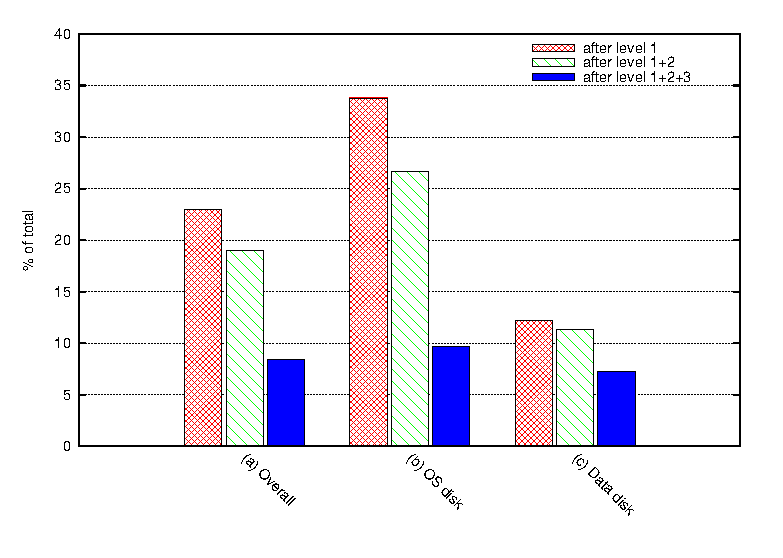
\epsfig{file=images/overall_effect.eps, width=3.5in}
%  \caption{Impacts of 3-level deduplication. The height of each bar is the data size after 
%deduplication divided by the original data size and the unit is percentage. }
%  \label{fig:overall}
%\end{figure}

%We assess the deduplication efficiency of VC and compare with
%that of an VO approach  using stateless routing with binning (SRB).
%SRB routes a data chunk to a machine~\cite{ParallelDataDomain}
%using  the chunk hashing function disussed in \cite{??}. 

Figure~\ref{fig:exbin-efficiency-graph} shows the deduplication efficiency for SRB and VC.
We define deduplication efficiency to be the percent of duplicate chunks
which are detected and deduplicated.
The figure also compares several PDS sizes chosen for VC. ``$\sigma=2\%$'' means that
we allocate the space of distributed shared memory  to accommodate 2\%
of data chunks shared among VMs, as defined in Table~\ref{tab:symbol}. Namely 
With $\sigma=2\%$, the deduplication efficiency can reach over 90\% 
while with $\sigma=4\%$, the deduplication efficiency can reach 92\%. 
The loss of efficiency in VC is caused by the restriction of the total physical memory available
in the cluster to support the PDS.  
The loss of efficiency in SRB is caused by the routing of data chunks which restricts the search scope
for global comparison.
In all cases, VC provides similar or better deduplication efficiency than SRB.

This result shows VC can remove  a competitive amount of duplicates.
In general, our experiments show that
dirty-bit detection at the segment level  can reduce the data size to about 23\% of original data, 
which leads  about 77\% reduction.
Local search within a segment can   further reduce the data size
to about 18.5\% of original size, namely it delivers additional 4.5\% reduction.
The PDS-based cross-VM detection with $\sigma=2\% $
can reduce the  size further to 8\% of original size, namely it 
delivers additional 10.5\% reduction.


\comments{%both of the bar charts are superceded by the graph below
%\comments{
    %this version of the figure is vertical
    \begin{figure}[ht]
  \centering
    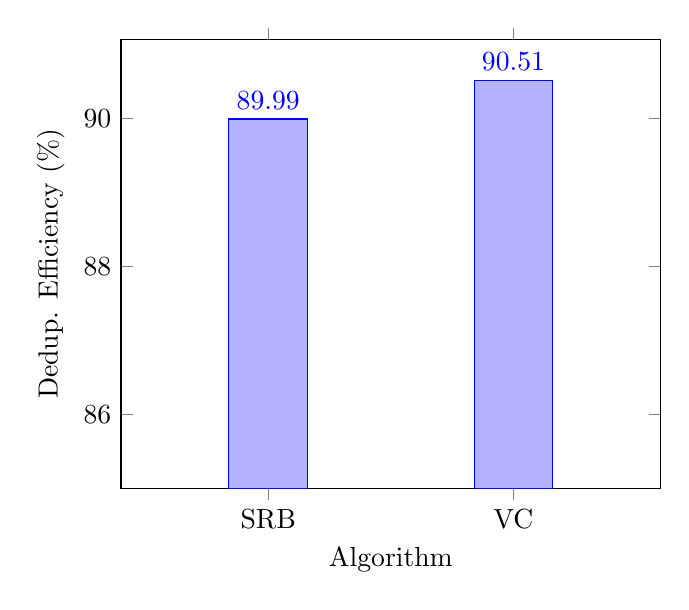
\begin{tikzpicture}
            \begin{axis}[
            %title={Extreme-Binning Efficiency},
            ybar,
            bar width=1.00cm,
            symbolic x coords={SRB,VC},
            xlabel={Algorithm},
            ylabel={Dedup. Efficiency (\%)},
            %extra y ticks={4.5,5.5,6.5} %to add extra ticks
            xtick=data, %without this the symbolic coords may be repeated as filler
            enlarge x limits=0.6, %used to push plots towards center
            ymin=85,
            %ymax=100,
            nodes near coords,
            nodes near coords align={vertical},
            ]
            \addplot coordinates {(SRB,89.99) (VC,90.51)};
            \end{axis}
    \end{tikzpicture}
    \caption{Deduplication Efficiency
         of SRB  and VC with $\delta=2\%$.}
        %($efficiency=\frac{d-du}{d-du_{complete}}$) comparison between Stateless Routing with Binning and VC with 2\% PDS.}
  \label{fig:exbin-efficiency1}
\end{figure}
%}
%same figure as above but horizontal (better for only two data points)
\begin{figure}[ht]
  \centering
    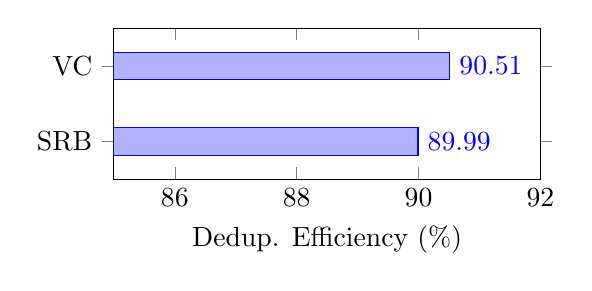
\begin{tikzpicture}
            \begin{axis}[
            %title={Extreme-Binning Efficiency},
            xbar,
            width=7cm,
            height=3.5cm,
            %bar width=0.75cm,
            symbolic y coords={SRB,VC},
            xlabel={Dedup. Efficiency (\%)},
            %ylabel={Algorithm},
            %extra x ticks={4.5,5.5,6.5} %to add extra ticks
            ytick=data, %without this the symbolic coords may be repeated as filler
            enlarge y limits=0.5,
            xmin=85,
            xmax=92, %otherwise label overlaps with right border
            nodes near coords,
            nodes near coords align={horizontal},
            ]
            \addplot coordinates {(89.99,SRB) (90.51,VC)};
            \end{axis}
    \end{tikzpicture}
    \caption{Deduplication Efficiency
        ($efficiency=\frac{d-du}{d-du_{complete}}$) comparison between Stateless Routing with Binning and VC with 2\% PDS.}
  \label{fig:exbin-efficiency2}
\end{figure}
}

\comments{%superceded by minhash algorithm (below)
%graph comparing extreme binning (SRB) with PDS model (VC) for different cds percentages
\begin{figure}[ht]
  \centering
    \begin{tikzpicture}
            \begin{axis}[
            %title={Ex-Binning Efficiency},
            cycle list name=mline,
            xlabel={Number of VMs added},
            ylabel={Dedup. Efficiency (\%)},
            %extra y ticks={4.5,5.5,6.5} %to add extra ticks
            mark options=solid,
            legend pos=south west,
            %legend columns=2,
            %legend style={
            %    at={(0.5,-0.2)},
            %anchor=north},
            ]
            \addplot table[x=VMs,y=exbin] {figures/exbin_efficiency_comparison.txt};
            \addplot table[x=VMs,y=cds4] {figures/exbin_efficiency_comparison.txt};
            \addplot table[x=VMs,y=cds2] {figures/exbin_efficiency_comparison.txt};
            \addplot table[x=VMs,y=cds1] {figures/exbin_efficiency_comparison.txt};
            \legend{SRB,VC ($\sigma=4\%$),VC ($\sigma=2\%$),VC ($\sigma=1\%$)};
            \end{axis}
    \end{tikzpicture}
    \caption{Deduplication Efficiency
        ($efficiency=\frac{d-du}{d-du_{complete}}$) comparison between
    SRB and  VC.}
  \label{fig:exbin-efficiency-graph}
\end{figure}
}

\comments{%version of above graph using minhash algorithm
\begin{figure}[ht]
  \centering
    \begin{tikzpicture}
            \begin{axis}[
            %title={Ex-Binning Efficiency},
            width=\linewidth,
            height=0.7\linewidth,
            cycle list name=mline,
            xlabel={Number of VMs added},
            ylabel={Dedup. Efficiency (\%)},
            xmin=0,
            ymin=88.5,
            ymax=100,
            %extra y ticks={4.5,5.5,6.5} %to add extra ticks
            mark options=solid,
            legend pos=south west,
            legend columns=2,
            legend style={
                font={\tiny},
                %at={(0.5,-0.2)},
                %anchor=north
            },
            ]
            \addplot table[x=VMs,y=exbin] {figures/exbin_efficiency_comparison2.txt};
            \addplot table[x=VMs,y=MHcds4] {figures/exbin_efficiency_comparison2.txt};
            \addplot table[x=VMs,y=MHcds2] {figures/exbin_efficiency_comparison2.txt};
            \addplot table[x=VMs,y=MHcds1] {figures/exbin_efficiency_comparison2.txt};
            \addplot table[x=VMs,y=MHNocds] {figures/exbin_efficiency_comparison2.txt};
            \legend{SRB,VC ($\sigma=4\%$),VC ($\sigma=2\%$),VC ($\sigma=1\%$),VC (No PDS)};
            \end{axis}
    \end{tikzpicture}
    \caption{Deduplication Efficiency
        ($efficiency=\frac{d-du}{d-du_{complete}}$) comparison between
    Stateless Routing with Binning and VC. VC uses the minhash algorithm for Level-2.}
  \label{fig-exbin-efficiency-graph2}
\end{figure}
}

%this version combines the old and the minhash alg. to compare against srb
\begin{figure}[ht]
  \centering
    \begin{tikzpicture}
            \begin{axis}[
            %title={Ex-Binning Efficiency},
            width=\linewidth,
            height=0.75\linewidth,
            cycle list={%
                {blue,solid,mark=square*},
                {blue,solid,mark=triangle*,mark size=1.5},
                {blue,solid,mark=diamond*,mark size=1.5},
                {blue,solid,mark=pentagon*,mark size=1.4},
                {red,draw=red,densely dotted,mark=square},
                {red,densely dotted,mark=triangle,mark size=1.5},
                {red,densely dotted,mark=diamond,mark size=1.5},
                {brown,densely dashed,mark=*},
                %{red,densely dotted,mark=o},
                %{red,densely dotted,mark=pentagon,mark size=1.4},
            },
            mark repeat={5},
            xlabel={Number of VMs added},
            ylabel={Dedup. Efficiency (\%)},
            xmin=0,
            ymin=88.5,
            ymax=100,
            %extra y ticks={4.5,5.5,6.5} %to add extra ticks
            mark options=solid,
            legend pos=south west,
            legend columns=2,
            legend style={
                font={\tiny\sffamily},
                %at={(0.5,-0.2)},
                %anchor=north
            },
            ]
            \addplot table[x=VMs,y=MHcds4] {figures/exbin_efficiency_comparison2.txt};
            \addplot table[x=VMs,y=MHcds2] {figures/exbin_efficiency_comparison2.txt};
            \addplot table[x=VMs,y=MHcds1] {figures/exbin_efficiency_comparison2.txt};
            \addplot table[x=VMs,y=MHNocds] {figures/exbin_efficiency_comparison2.txt};
            \addplot table[x=VMs,y=cds4] {figures/exbin_efficiency_comparison.txt};
            \addplot table[x=VMs,y=cds2] {figures/exbin_efficiency_comparison.txt};
            \addplot table[x=VMs,y=cds1] {figures/exbin_efficiency_comparison.txt};
            \addplot table[x=VMs,y=exbin] {figures/exbin_efficiency_comparison2.txt};
            \legend{VC MH( $\sigma=4\%$),VC MH($\sigma=2\%$),VC MH($\sigma=1\%$),VC MH(No PDS),VC($\sigma=4\%$),VC($\sigma=2\%$),VC($\sigma=1\%$),SRB};
            \end{axis}
    \end{tikzpicture}
    \caption{Deduplication Efficiency
        ($efficiency=\frac{d-du}{d-du_{complete}}$) comparison between
    Stateless Routing with Binning and VC. Also compares old VC algorithm to new VC with Minhash for Level-2.}
  \label{fig-exbin-efficiency-graph2}
\end{figure}

%\begin{figure}
%  \centering
 %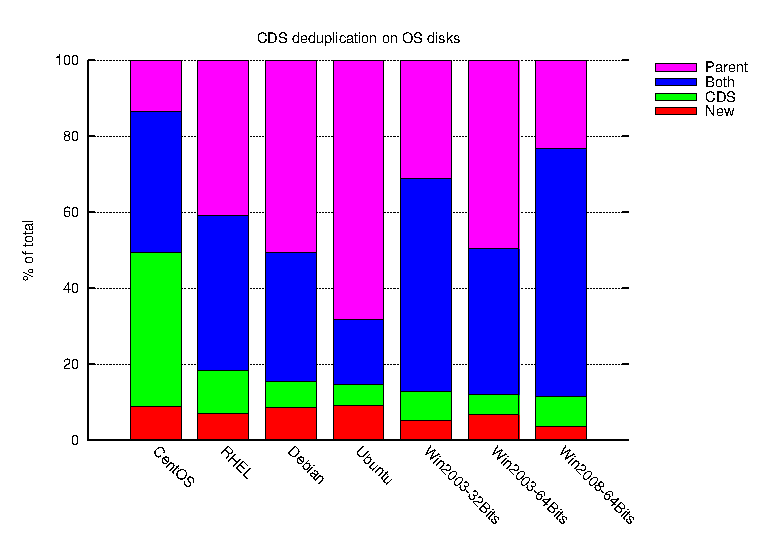
\epsfig{file=images/os_cds_sim.eps, width=3in}
%  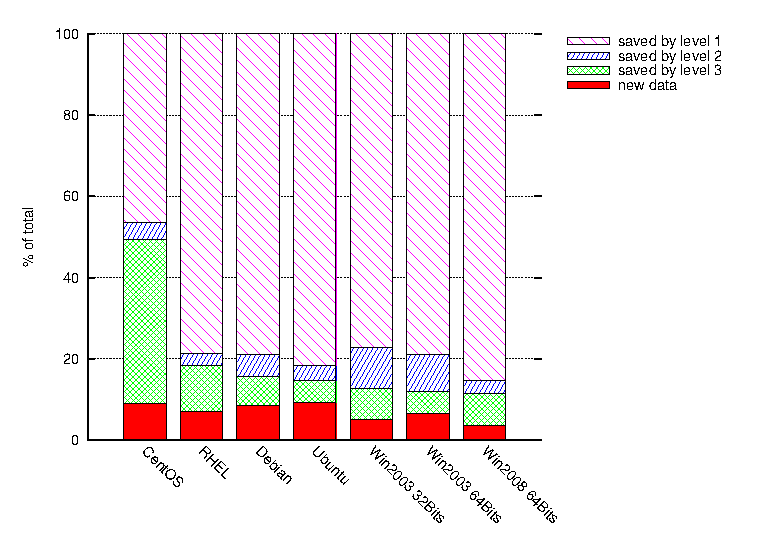
\epsfig{file=images/3level_os.eps, width=3.5in}
%  \caption{Impact of 3-level deduplication for OS releases.}
%  \label{fig:oscds}
%\end{figure}

%To see the impact of multi-level deduplication on different OS releases,
%Some of  OS disks are modified frequently and in some cases,  users even store a large amount of user data on

%Combining OS disks in all the VMs, we see the overall 7.4TB of data is reduced to 512GB. 
%The extreme binning approach can reduce this data set to 542GB, which is slightly worse. As a reference, 
%perfect deduplication achieves 364GB in this experiment.

%Overall speaking, inner   VM deduplication or  PDS-based deduplication
%can work well alone, but by combining them together we get a fairly good and stable deduplication ratio to 
%all kind of OSes. 
%Compared to a traditional dirty bit approach based on pages of
%each file (e.g. segment in our scheme),
%our PDS-based level 3 approach  can save additional 50\% storage space because many of level 2 block
%content can be eliminated using the PDS also.

\subsection{Resource Usage}
{\bf Storage cost of replication.}
\begin{table}
    \begin{tabular}{|c|c|}
    \hline
    PDS replication degree & Total space (GB) \\ \hline
    3                      & 3065             \\ \hline
    4                      & 3072             \\ \hline
    5                      & 3079             \\ \hline
    6                      & 3086             \\ \hline
    7                      & 3093             \\ \hline
    \end{tabular}
\caption{Storage space cost under different PDS replication degree}
\label{tab:replication_cost}
\end{table}

Table~\ref{tab:replication_cost} shows the total storage space required by VC as the PDS replication degree is changed. The increase in storage cost is minimal because the PDS makes up a very small percent of the total storage space, but the increase in reliability can be much more significant (see Figure~\ref{fig:pds-replication}).

\begin{table}
    \begin{tabular}{|c|c|c|c|c|}
    \hline
    Tasks & CPU & Mem (MB) & Disk W (MB/s) & Network \\ \hline
    1                      & 19\% & 18.1 & 32.1     &    \\ \hline
    2                      & 35\% & 31.8 & 53     &    \\ \hline
    4                      & 63\% & 54.1 & 84     &    \\ \hline
    6                      & 77\% & 71.9  & 88.5   &     \\ \hline
    8                      & 82\% & 90.5   & 89.2   &    \\ \hline
    10                      & 85\% & 97.2   & 90.4   &    \\ \hline
    12                      & 91\% & 95.6    & 91.5   &   \\ \hline
    \end{tabular}
\caption{Resource usage under concurrent backup tasks}
\label{tab:resource_usage}
\end{table}


\subsection{Processing Time and Throughput}
%{\bf Single VM Backup} We start the evauluation of our system by examine the normal warmed-up
%backup scenario - taking a snapshot of a VM which already has old backups exist. To simulate this
%scenario, we pick one 40GB VM from the data set, make an initial snapshot backup, then
%evaulate the system performance on the second snapshot backup. We repeat such procedure
%under different PDS memory usage settings, the results of backup time break down are shown in

Figure~\ref{fig:srb_vs_vc} shows
the  average  processing  time of  each segment using VC and SRM in handling our dataset.
It has a breakdown of time for reading data and updating the metadata, network latency to visit
a remote machine, and index access for finger printer comparison.
SRB has a higher index access and fingerprint comparison because once a chunk is routed to a machine,
it relies on this local machine to access its index (often on the disk) and perform comparison.
VC is faster for index access because it conducts in-memory local search first and then
accesses  the PDS which is on distributed shared memory.  
SRB spends  slighter more time in  reading data and updates because it also updates the on-disk
local meta data index.
Overall,  VC is faster than SRB, though data reading dominates the processing time for both algorithms.
%all lookups are essentially random and caching will be largely innefective).  

%\emph{Should we use one of the two
%bar charts, or the graph? I am thinking the graph, but I'll leave the two bar
%charts in the paper until we decide? If we use the bar charts some text will
%have to be changed. We could also add each of the PDS sizes to the bar chart
%and have 4 bars instead of 2.}

\begin{figure}[htbp]
  \centering
  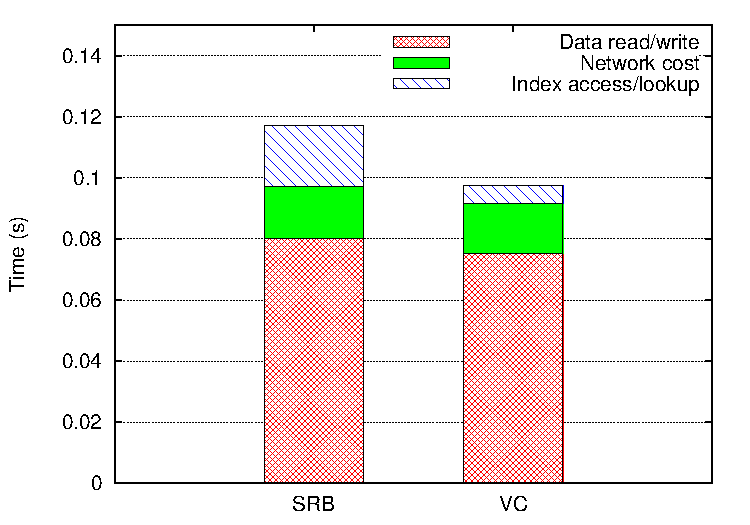
\epsfig{file=figures/srb_vs_vc, width=3.5in}
  \caption{Time to backup a dirty segment under SRB and VC approach}
  \label{fig:srb_vs_vc}
\end{figure}

Figure~\ref{fig:single_vm_backup} reports the average bacup time for a VM in VC with a varying PDS size.
Again it shows that data reading dominates the backup process; our deduplication
procedure only takes a small fraction of the total backup time. 
The change of $\sigma$ does not significantly affect the overall backup speed as
PDS lookup takes only a small amount of time.
%Larger memory permits us to
%use larger PDS index to cover more of global index, as a result the amount of data to be writen
%is reduced and so do the writing time.
%Inside the deduplication procedure, the time costs of level-1
%is plainly zero, and the costs of level-2 and level-3 are almost identical under different settings
%because the number of fingerprints to process are just the same.


\begin{figure}
    \centering
    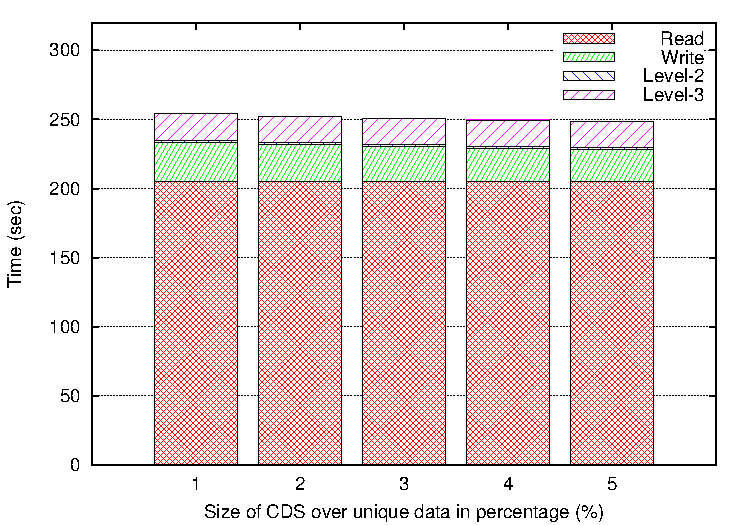
\includegraphics[width=3in]{figures/single_backup_time}
    \caption{Backup times for varying PDS sizes}
    \label{fig:single_vm_backup}
\end{figure}


    Figure~\ref{fig:parallel_backup} shows the node throughput when all machine nodes run
the backup procedure in parallel.
To begin, on each node we write snapshots for 4 VMs concurrently, and gradually 
increase number of VMs to 12 to saturate our system capability. We observed 
the per-node throughput peaked at 2700 MB/s when writing 10 VM snapshots in parallel, 
which is far beyond our QFS file system capability. The reason behind it is our efficient
deduplication architecture and compression which greatly reduce the amount of data that needs to be written to
the file system. The main bottleneck here is that our QFS installation only
manages one disk per node, which prevents it from fully utilizing the the
benefits of parallel disk access. We expect our architecture can
perform even better in production clusters, which often have ten or more disks on each node.



\begin{figure}
    \centering
    \subfigure[Real VM backup performance]
    {
        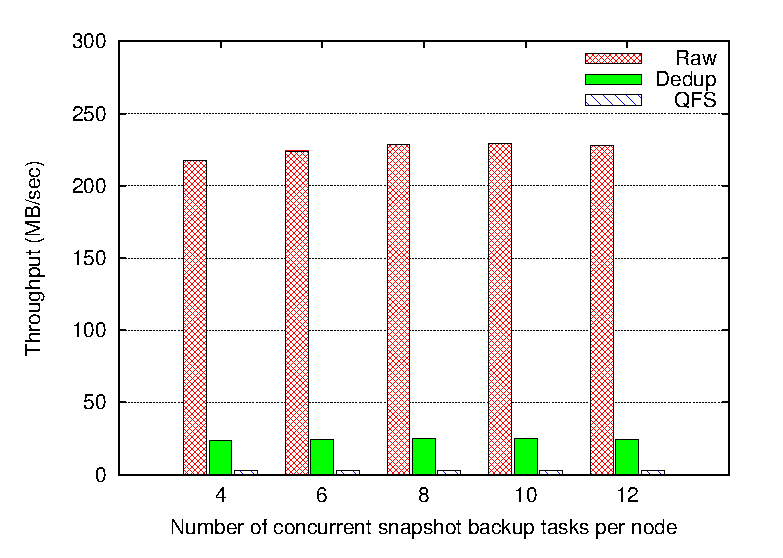
\includegraphics[width=3in]{figures/parallel_backup_with_read}
        \label{fig:withread}
    }
    \\
    \subfigure[Deduplication and storage system performance]
    {
        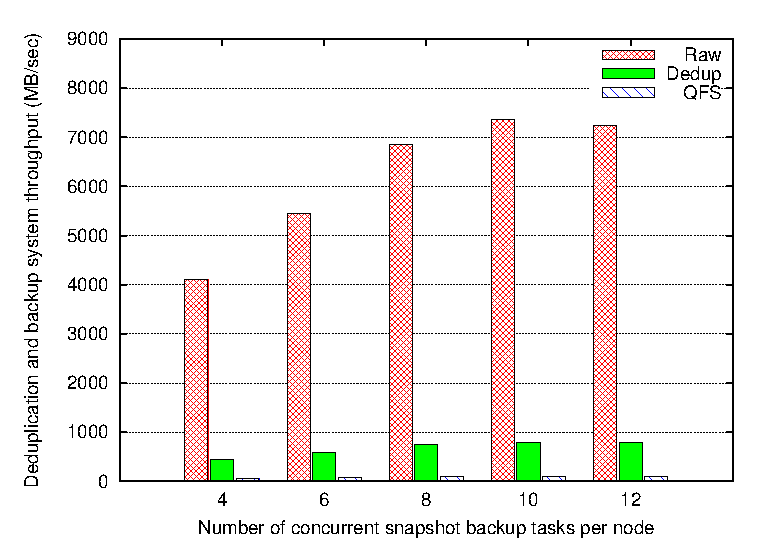
\includegraphics[width=3in]{figures/parallel_backup_no_read}
        \label{fig:noread}
    }
    \caption{Throughput per-node with concurrent snapshot backup tasks}
    \label{fig:parallel_backup}
\end{figure}


% \begin{figure}[htbp]
%   \centering
%   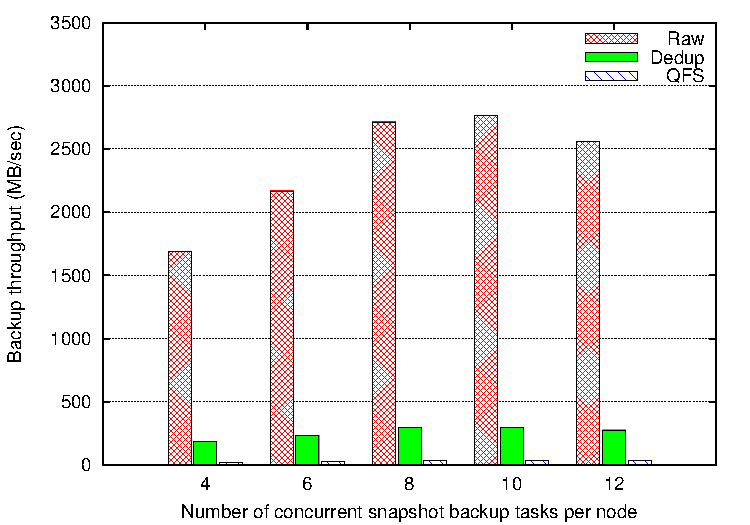
\epsfig{file=figures/parallel_backup, width=3.5in}
%   \caption{Throughput per-node with concurrent snapshot backup tasks}
%   \label{fig:parallel_backup}
% \end{figure}


% \begin{table}
% \begin{tabular}{ |p{1.5cm}|p{1.8cm}|p{1.2cm}|p{1.4cm}| }
% \hline
%  & Costs & Stateless routing with binning (s) & VM-centric approach (s) \\ \hline
% \multirow{4}{*}{\vbox{I/O related}} & Read data & 0.05 & 0.05 \\ \cline{2-4}
%  & Transfer data  & 0.017 & 0.017 \\ \cline{2-4}
%  & Write data & 0.03 & 0.025 \\ \cline{2-4}
%  & Subtotal & 0.097 & 0.092 \\ \hline
% \multirow{5}{*}{\vbox{Dedupe related}} & Read index/recipe & 0.01 & 0.00045 \\ \cline{2-4}
%  & Write index/recipe & 0.01 & 0.0051 \\ \cline{2-4}
%  & Transfer fingerprints & 0.00058 & 0.00013 \\ \cline{2-4}
%  & PDS lookup & N/A & 0.00034 \\ \cline{2-4}
%  & Subtotal & 0.021 & 0.0064 \\ \hline
% \multicolumn{2}{ |c| }{Total} & 0.12 & 0.098 \\
% \hline
% \end{tabular}
% \caption{Time of backup a segment break down}
% \label{tab:compare}
% \end{table}
\subsection{Approximate Deletion}

\begin{figure}
    \centering
    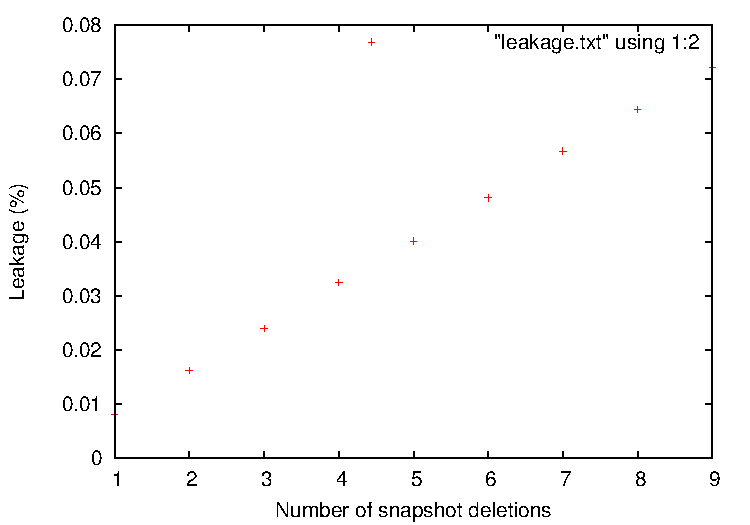
\includegraphics[width=3in]{figures/leakage}
    \caption{Accumulated storage leakage by approximate snapshot deletions}
    \label{fig:leakage}
\end{figure}

Figure\ref{fig:leakage} shows the average accumulated storage leakage resulted by daily
approximate deletions among all VMs. We see the storage leakage ratio is satisfactory: 
after 9 snapshot approximate deletions, there is only 1MB space leaked over every 10GB
of stored data. In addition, the leakage ratio grows linearly with the number of approximate deletions
as our analysis, which gives us a reliable prediction of when to trigger a accurate mark-and-sweep delete operation. 
  

\comments{
\subsection{Read Snapshot}

\subsection{Comparison with Other Approaches}
\subsubsection{Sampled Index}
One alternative approach to avoiding a single global index is to use a sampled
index. This is the approach taken by Guo and Efstathopoulos\cite{Guo2011}. We
compare their solution to ours by running their algorithm on our 350 traces
using a sampling rate of 1 out of 101 blocks, and always including the first
block in a container (which we fix at 16MB in size). The results of running this
test are shown in Table~\ref{??}, and the memory usage comparison can be found
Sec.~\ref{??}. Our results show that using a sampled index achieves a very high
rate of deduplication, and so a sampled index might be a good way to do dedup
in a single node setup.

The problems for sampling are in distributing the
algorithm and in deduplicating extremely large bodies of data. The algorithm
stores the entire (sampled) index in memory, which is required for high
throughput to avoid the disk-bottleneck problem - since the index itself has no
locality information, lookups are essentially random, so the index must be
somehow optimized to prevent excessive disk seeking (the sampling algorithm does
this by storing the index in memory). To distribute this index, each node would
either require a complete copy of the index which would have a prohibitive cost in
memory, or something like memcached must be used, which leaves the same problem
as the disk bottleneck with every index check potentially using the network.
The difficulty in storing extremely large bodies of data
is related, as once 1PB is stored in the system, assuming a sampling rate of 
1/101 with 22 byte index entires, 55GB of (in memory) index are required.

Our solution uses more total memory (??how much??), but is more scalable both in
terms of capactity and distributing the deduplication. The only part of our
algorithm which requires significant network traffic is the PDS deduplication,
but this is done after Levels 1 and 2 (dirty bits and comparison to parent), and
so is only done for a small percent of blocks (?? 5-10\% ??).

\subsubsection{Scalable Data Routing}
Another approach to avoiding a global index is to use a content-based hash
partitioning algorithm to break up the deduplication work. This approach is
taken by Dong et al. in their Scalable Data Routing paper, and is similar to
Exreme Binning\cite{??}\cite{extreme_binning09}. We compared our solution to
content-based hash partitioning by running the algorithm on our set of 
traces. We used 2MB superchunks and 4KB chunks to partition the data, and use
the minhashes of the superchunks for routing. The results of this are shown in
Table~\ref{??}. Routing each chunk to a bin provides good deduplication
efficiency, and only requires each storage node to keep an index of local data
and the bin mapping, but misses significant opportunities in our indended use
case.

The problem with the Data Routing algorithm is in the very high network traffic.
Our intended use case is a backup system which runs alongside a number of VMs,
in order to save costs. Data Routing makes no use of the inherent locality in
such a system, and therefore puts a much higher network burden on machines which
are also running 35 VMs each. This will reduce the available network bandwidth
to users of the VMs, and/or reduce the possible deduplication throughput.

}
